\hypertarget{gestion_copias_de_seguridad}{}
\chapter{Gestión de copias de seguridad (backups)}

\section{Introducción}

Una copia de seguridad, o \textbf{\textit{backup}}, \textbf{es una copia de los datos originales} que se realiza con el fin de disponer de un medio \textbf{para recuperarlos en caso de pérdida}. Las copias de seguridad son útiles en caso de que los datos originales se hayan perdido por un fallo humano, fallo de sistema (rotura de disco duro), modificado por un virus,  evento natural (incendio del edificio), un ataque (borrado deliberado de los datos), etc…

El proceso de copia de seguridad también tiene que tener en cuenta el método de “\textbf{restauración de los datos}”, que es el momento en el que necesitaríamos realizar la restauración de los datos del \textit{backup} para dejarlos en la ubicación original.

A la hora de pensar un sistema de copias de seguridad, tendremos que tener en cuenta los siguientes puntos:

\begin{itemize}
    \item Importancia de los datos
    \item Espacio ocupado por la copia de seguridad
    \item Ubicación de la copia de seguridad
    \item Plan de recuperación ante desastre
    \item Punto máximo que podemos recuperar
    \item Tiempo estimado de recuperación de los datos
\end{itemize}

Por otro lado, también tendremos que tener en cuenta el método que vamos a utilizar para realizar la copia de seguridad, y cómo va a ser el proceso. Este proceso dependerá del servicio/sistema al que vayamos a realizar el backup.

Y por último, la estrategia a utilizar:

\begin{itemize}
    \item Estrategia multi-backup completos
    \item Incrementales y/o diferenciales
    \item Estrategia personalizada
    \item La que el programa que vayamos a utilizar nos permita
    \item …
\end{itemize}

Antes de realizar la copia de seguridad de los datos tendremos que tener muy en cuenta distintos apartados, que deberán ser analizados en detalle y puede que modificados en el futuro.

\section{A tener en cuenta}
Durante la \textbf{planificación} de la creación de las copias de seguridad hay ciertos aspectos que tenemos que tener en cuenta para que la gestión de copias de seguridad se realice de manera satisfactoria.

Esta planificación debe realizarse conociendo los datos que maneja la empresa, la importancia de los mismos, el volumen que ocupan, la cantidad de cambios que reciben, ...

\infobox{Una buena planificación para la gestión de copias de seguridad de una empresa puede involucrar a varias personas de distintos ámbitos internos.}

\subsection{Conocer los datos y la importancia de los mismos}
Para saber sobre qué datos tenemos que realizar las copias de seguridad, debemos conocer los datos que manejamos en la empresa, la importancia que tienen y su ubicación. \textbf{Ejemplo}: no es lo mismo la importancia de los datos gestionados en la base de datos de clientes, o el directorio “Descargas” el PC de un usuario.

También tendremos que conocer el tamaño actual de esos datos, y saber cuánto volumen total alcanzan. Cuanto mayor tamaño tengan, también mayor será el espacio ocupado por las copias de seguridad.


Otro aspecto a tener en cuenta es saber las modificaciones que sufren esos datos, y estimar el volumen de esos cambios. \textbf{Ejemplo}: no es lo mismo que una base de datos reciba 10 clientes nuevos al día o que reciba 15.000 ventas a la hora en nuestra tienda online.


\infobox{\textbf{Debemos conocer los datos que existen en nuestra empresa, la ubicación, la importancia y el volumen que ocupan para así poder realizar un buen plan de gestión de copias de seguridad.}}

\subsection{Espacio ocupado por la copia de seguridad}
Estimar el espacio que nos va a ocupar una copia de seguridad puede parecer sencillo, pero no siempre es así, y es por eso que conocer los datos, tal como hemos dicho antes, es de vital importancia.

Tendremos que tener en cuenta cuánto ocupan nuestros datos originales, cuál va a ser la estrategia de backup a utilizar, estimar el incremento de espacio que puede haber en los datos originales…

Por lo tanto, siempre deberíamos estimar por alto el espacio ocupado, y siempre pudiendo realizar la expansión de ese espacio “en caliente”, para que las copias de seguridad funcionen cada día.

\errorbox{\textbf{No realizar copias de seguridad debido a falta de espacio debería ser considerado un fallo de primer orden y que debe ser subsanado lo antes posible.}}


\subsection{Punto mínimo en el tiempo que queremos recuperar}
Es posible tener copias de seguridad que estén completamente actualizadas en cuanto se realizan cambios en los datos originales, pero la puesta a punto de estos sistemas puede no estar a nuestro alcance (por no conocer cómo se realizan o por un coste elevado).

En ciertos casos, algunas empresas pueden aceptar la pérdida de ciertos datos, ya que el gestionar que las copias se realicen “en tiempo real” es más caro que el repetir el proceso de crear esos datos de nuevo.

\textbf{Ejemplo}: Una empresa puede no necesitar hacer backup de la base de datos de cuándo fichan los empleados en tiempo real, porque si se pierden los datos de un día es asumible (el backup se hace cada noche). En cambio, la base de datos de marketing tiene que realizarse en tiempo real.


\subsection{Punto máximo en el tiempo que queremos recuperar}
Otro aspecto importante a tener en cuenta es \textbf{pensar cuánto tiempo para atrás queremos poder llegar para poder realizar la restauración de los datos}. No será lo mismo querer realizar una restauración de los datos de hace una hora, un día, de hace una semana o de hace un año, ya que esta decisión influirá en toda estrategia de copia de seguridad.

Es por eso, que a los datos hay que darle la importancia que se merece, y es bastante probable que distintos datos tengan distintos puntos de restauración máximo.

\textbf{Ejemplo}: No es lo mismo los datos de facturación de una empresa, que la ley nos marca que debemos guardar dichos datos (4 años), los datos de una página web que apenas cambia (igual nos sirve una copia a la semana) o la carpeta personal de un usuario en su equipo (dado que en su equipo no debería guardar nada importante de la empresa, se podría asumir una pérdida de datos).


\subsection{Ubicación de la copia de seguridad}
Es muy importante también tener en cuenta cuál va a ser la ubicación de la copia de seguridad y las consecuencias que eso puede conllevar.
 Vamos a poner varios ejemplos:

\begin{itemize}
    \item Si decidimos hacer la copia de seguridad en el mismo equipo informático, un problema de electricidad podría suponer la pérdida de los datos originales y los backups.
    \item Si decidimos realizar la copia de seguridad en la misma sala de ordenadores donde se sitúan los datos originales, si esa sala se ve involucrada por un factor que destruya todo (un incendio, un robo, …), perderíamos todos los datos.
    \item Si decidimos realizar la copia en la misma oficina, edificio, puede pasar lo mismo que el punto anterior
    \item Si decidimos realizar la copia en la “nube”, el tiempo para realizar la copia de seguridad y el tiempo de restauración de los datos puede incrementarse
    \item Si decidimos realizar la copia en otra oficina, dependemos de la conexión, los datos deberían ir cifrados, tiempo de creación de la copia de seguridad y restauración…

\end{itemize}
Como se puede ver, cada ejemplo puede tener unos pros y unos contras.

\errorbox{\textbf{La copia de seguridad nunca debería estar en el mismo equipo informático, y mucho menos en el mismo disco duro físico, que los datos originales.}}

\subsection{Tiempo estimado de la copia}
Teniendo en cuenta lo comentado previamente, el tiempo estimado de la copia de seguridad es muy importante, y es posible que varíe en el tiempo. No es lo mismo realizar la copia de seguridad de unos pocos megabytes o de varios gigabytes.

Es por eso por lo que tendremos que tener en cuenta el tiempo que tarda en realizarse nuestras copias de seguridad para así asegurar que se realizan de manera correcta y no se solapan en el tiempo.


\subsection{Plan de recuperación ante desastre}
Tan importante es tener una copia de seguridad como un plan ante un posible desastre. De nada sirve tener una copia de seguridad si restaurarla nos va a llevar semanas por no saber el estado de las mismas, o si su restauración es compleja.

Por lo tanto, \textbf{es muy importante disponer de un plan de recuperación ante desastres que esté actualizado}, que contemple si ha habido modificaciones en la gestión de copias de seguridad, que tenga en cuenta los pasos a realizar…

Este plan de recuperación \textbf{debería ser puesto en práctica cada cierto tiempo para asegurar que sigue estando vigente}, y si no, realizar las modificaciones oportunas.

\warnbox{\textbf{Es muy importante disponer de un plan de recuperación ante desastres que esté actualizado y probar que siga vigente cada cierto tiempo.}}

El plan de recuperación ante desastre debería contener:
\begin{itemize}
    \item Los distintos métodos y estrategias de copias de seguridad que existen en la empresa
    \item Ubicaciones donde se realizar las copias de seguridad
    \item Importancia de los datos de los que se realizar la copia de seguridad
    \item Cómo realizar la restauración de cada sistemas de los que se ha realizado la copia de seguridad
    \item Orden para realizar las restauraciones y dada la importancia de los datos, la prioridad de las restauraciones
    \item ...
\end{itemize}

\infobox{El plan de recuperación es algo que toda compañía debe tener a la hora de crear sus sistema de copias de seguridad, ya que deben de ir de la mano.}

\subsection{Tiempo estimado de recuperación de los datos}
El último punto, pero no por ello menos importante, es el tiempo estimado de recuperación de los datos.

\errorbox{\textbf{De poco sirve tener copias de seguridad y un plan de recuperación, si luego es posible que estemos dos semanas para recuperar los datos.}}

Es por eso que tenemos que conocer el tiempo estimado de recuperación de los datos para poder gestionar los tiempos con los empleados, los clientes…

Este tiempo estimado, al igual que el tamaño de las copias, puede variar en el tiempo, por lo que \textbf{debemos asegurar cada cierto tiempo el realizar simulacros para asegurar qué tiempos se manejan}.

\begin{center}
    \vspace{-15pt}
    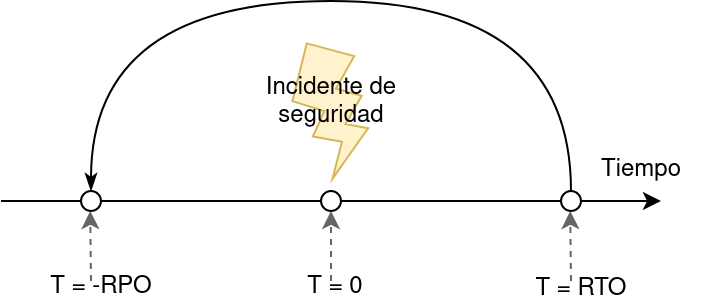
\includegraphics[width=0.6\linewidth]{incidente_seguridad.png}
    \vspace{-20pt}
\end{center}

Teniendo en cuenta el gráfico anterior:
\begin{description}
    \item[RTO:] es el objetivo de tiempo de recuperación (\textit{Recovery Time Objective}), y es el tiempo que se tarda en restablecer el servicio, o al menos los mínimos acordados. Cuanto menor sea el tiempo de recuperación, mejor.
    \item[RPO:] es el objetivo de punto de recuperación (\textit{Recovery Point Objective}), y es el último instante de tiempo previo al incidente al que los sistemas son capaces de regresar. Habitualmente suele ser marcado por la frecuencia con que se realicen las copias de seguridad. De nuevo, cuanto más cercano a T=0 mejor.
\end{description}


\section{Métodos de Backup}
Existen distintas estrategias a la hora de crear un backup, por lo que tendremos que analizar los datos que queremos salvaguardar y decidir la mejor estrategia.

\subsection{Copiar los ficheros}
Sería la metodología más sencilla. Simplemente haremos una copia de los datos importantes en otra ubicación/soporte. Este sistema hace que cada X tiempo, se guarden los ficheros y obtendremos una copia completa de los datos.

El problema es que \textbf{no tendremos la posibilidad de recuperar un fichero en un estado anterior a la última copia}. Es decir, si se realiza la copia de seguridad a las 6:00 de la mañana, no podremos obtener el estado del fichero previo a ese. Si a las 11:00 el usuario corrompe el fichero, podríamos recuperar al estado de las 6:00, pero no al estado de ayer.

\subsection{Sistema incremental a nivel de bloque}
Se basa en copiar sólo los bloques físicos que han sido modificados. Tendremos que tener guardado el fichero original por un lado, y a partir de ahí sólo guardaremos las modificaciones de manera incremental.

Para recuperar el fichero, primero tendremos que elegir restaurar el fichero original completo, y posteriormente aplicar los bloques incrementales hasta llegar al punto de restauración que nos interesa.

\subsection{Sistema incremental o diferencial binaria}
Similar al anterior, pero esta vez en lugar de hacer uso de bloques (1K, 4K, 8K…), la parte incremental o diferencial sería a nivel binario.

\subsection{Versionado de ficheros}
El versionado de ficheros se puede realizar de distintas maneras:

\begin{itemize}
    \item \textbf{Utilizando el sistema de ficheros}: Existen sistemas de ficheros que cuando uno es modificado, automáticamente crea una versión nueva del mismo.
    \item \textbf{Versionado manual}: cuando el usuario quiere crear una nueva versión del fichero, debe ejecutar a mano una acción para guardar la nueva versión del mismo.
\end{itemize}

\section{Estrategias de backup}
Existen muchas estrategias a la hora de realizar una copia de seguridad, quizá tantas como entornos existen, ya que se pueden utilizar estrategias generales o crear una para cada caso concreto. Vamos a explicar las más habituales.

\subsection{Multi-backup completos}
Este método sería el más sencillo, pero también el que más espacio nos ocuparía, y posiblemente el que más tiempo puede tardar, dependiendo de los datos a copiar.

En este método, podríamos hacer una copia completa de los datos que queremos guardar en tantas ubicaciones como queramos. Supongamos que queremos poder llegar a restaurar hasta 3 días de un fichero corrupto, eso supondría que tendríamos que tener 3 ubicaciones distintas donde cada día haríamos un backup completo de los datos. Por ejemplo:

\begin{itemize}
    \item Ubicación \textbf{1}: el \textbf{lunes} haríamos el primer backup completo
    \item Ubicación \textbf{2}: el \textbf{martes} haríamos el segundo backup completo
    \item Ubicación \textbf{3}: el \textbf{miércoles} haríamos el tercer backup completo
    \item Ubicación \textbf{1}: el \textbf{jueves} haríamos el backup completo (machando los datos previos que había del lunes)
    \item …
\end{itemize}

Como se puede ver, es una estrategia cíclica, sencilla, y que en ciertos casos puede ser más que suficiente. Pero como se ha comentado previamente, cada día se realizará un backup completo, por lo que habrá que tener en cuenta el tiempo que tarda, el espacio que ocupa, ...


\subsection{Incrementales y/o diferenciales}
Normalmente es el método más habitual y todos los programas suelen tener estos métodos a la hora de realizar copias de seguridad.

El hacer uso de copias incrementales y/o diferenciales nos permitirá poder restaurar los datos hasta un punto concreto. Por eso será muy importante tener en cuenta cuánto tiempo queremos poder llegar a restaurar, porque no es lo mismo a la hora de estimar espacio ocupado, si queremos restaurar los datos de una semana, de hace un mes o de hace un año.

Por lo tanto, a la hora de utilizar esta metodología, como ya se ha comentado, que es la más habitual, la estimación de espacio debe de ser holgada, y pensar a futuro, en cuánto puede llegar a aumentar el espacio ocupado.

\subsubsection{Incrementales}
Supongamos que realizamos una copia completa de los datos el domingo, esta será la base para las siguientes copias incrementales de los datos:

\begin{center}
    \vspace{-10pt}
    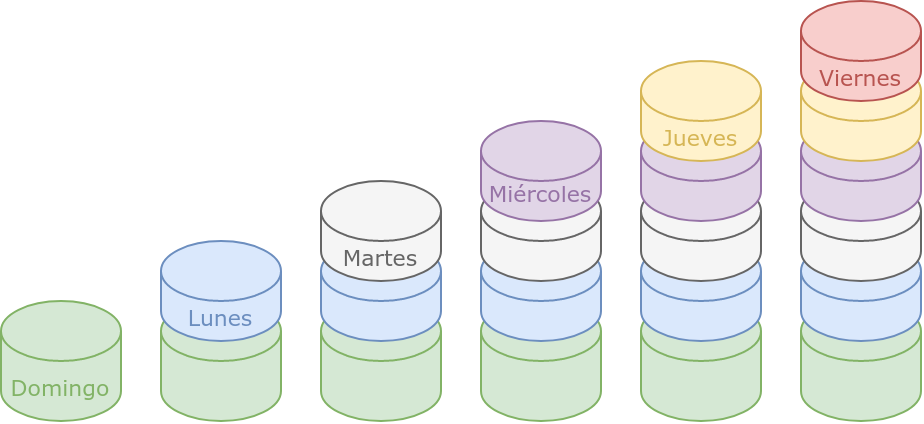
\includegraphics[width=0.7\linewidth]{incremental.png}
    \vspace{-20pt}
\end{center}

El lunes se hará una copia guardando sólo los datos que han cambiado respecto a la copia del domingo. El martes, se hará una copia de los datos que han sido modificados desde la copia del lunes… Y así sucesivamente.

Este método es rápido, fácil de realizar y sabemos claramente cuándo se han modificado los datos, por lo que si tenemos cada incremental separado en distintas carpetas, la restauración sería también sencilla.

\subsubsection{Diferencial}
Similar al incremental, pero cada día se guarda todos los datos que han sido modificados desde el último backup completo:

\begin{center}
    \vspace{-10pt}
    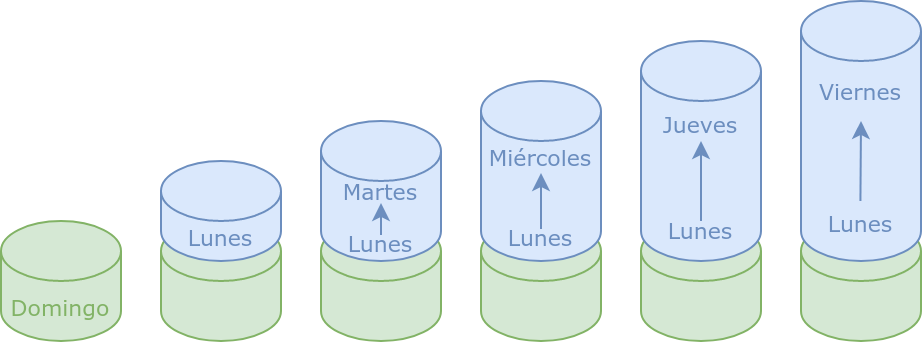
\includegraphics[width=0.7\linewidth]{diferencial.png}
    \vspace{-20pt}
\end{center}

Esto hace que cada backup diferencial pueda ocupar más que un incremental, pero cada día obtendremos todos los cambios desde el último backup completo.

\subsubsection{Incremental y diferencial}
También suele ser habitual realizar la mezcla de ambas estrategias:
\begin{itemize}
    \item El primer domingo de cada mes realizar la copia completa.
    \item Hacer uso del método incremental de lunes a sábado
    \item Los domingos realizar un diferencial de toda la semana.
\end{itemize}

\subsection{Estrategia personalizada}
Como se ha comentado previamente, pueden existir tantas estrategias como entornos existan, por lo que dependiendo de nuestros datos, nuestro entorno, nuestro modelo de negocio, tendremos que crearnos una estrategia propia.

Este método puede ser el más complejo, ya que quizá tengamos que realizarlo a mano, pero con ello nos aseguraremos de darle la importancia que se merece a cada parte de los datos que tengamos que realizar un backup.

\subsection{La que el programa nos marque}
Si hacemos uso de un programa de gestión de backups, al final estaremos limitados a lo que el programa nos permita. Como se ha comentado, la estrategia incremental/diferencial suele ser la más ampliamente utilizada, por lo que casi todos los programas deberían tener esta opción.

Dependiendo del programa, nos permitirá hacer mezclas de estrategias, realizar copias a sistemas remotos (la nube, por FTP, SSH…), varios cada día… Por lo que quedaría en nuestra mano analizar distintos programas y ver cuál es el que mejor se adecúa a nuestras necesidades.


\section{Regla 3-2-1}
Con todo lo dicho anteriormente, una de las estrategias más habituales, de manera generalizada y simplificada, es la conocida como la “\textbf{Regla 3-2-1}”.

Esta regla se resume en:
\begin{itemize}
    \item \textbf{3 copias completas} de los datos.
    \item En \textbf{2 tipos de almacenamiento distintos}
    \item \textbf{1 de las copias debe estar fuera}
\end{itemize}

Imaginemos una base de datos de una tienda online que está situada en un servidor en un RACK junto con otros servidores nuestros en un proveedor contratado. En esta base de datos tenemos \textbf{los datos originales}.

Haremos uso de otro de los servidores del RACK en el que realizaremos una copia de seguridad completa. Esta será la \textbf{segunda copia completa}, que está en otro servidor y que podremos acceder de manera rápida a ella.

La \textbf{tercera copia} de los datos la tendremos en nuestra oficina, ya que realizaremos una copia remota de los datos. Esta tercera copia está situada fuera del proveedor contratado, por lo que si en ese CPD hubiese un incendio, tendríamos una copia en local.


\section{Realización de simulacros de recuperación de los datos}
\textbf{De nada sirve lo comentado hasta ahora, si no se realizan simulacros de desastre} y de recuperación de los datos para asegurar que todo funciona de manera correcta. Desgraciadamente, \textbf{también puede haber fallos en los sistemas de backups}, por lo que aunque creamos que se están realizando correctamente, quizá el día que vayamos a necesitarlos nos damos cuenta que no es así, por lo que no podríamos realizar la recuperación de datos.

\errorbox{\textbf{Deberíamos crear simulacros de desastre para asegurar que todos los eslabones de la cadena de nuestro sistema de copias de seguridad es funciona de manera correcta.}}

Estos simulacros nos deberían ayudar a asegurar que:

\begin{itemize}
    \item Las copias de seguridad funcionan de manera correcta
    \item Podemos realizar restauraciones de los datos a fecha que nos interesa
    \item El plan de recuperación ante desastre está actualizado y es funcional
    \item El tiempo estimado de recuperación es el adecuado
    una vez restaurados los datos, nuestro sistema es funcional y podemos seguir con la actividad comercial
\end{itemize}

\warnbox{\textbf{Si alguno de los puntos anteriores falla y no es correcto, deberemos repasar todo el plan estratégico de copias de seguridad para solventar los fallos, y así poder volver a realizar un nuevo simulacro para confirmar que esta vez es correcto.}}



\clearpage